\section{CMasked\-Value\-Predicate$<$ T $>$  Class Template Reference}
\label{classCMaskedValuePredicate}\index{CMaskedValuePredicate@{CMasked\-Value\-Predicate}}
{\tt \#include $<$CMasked\-Value\-Predicate.h$>$}

Inheritance diagram for CMasked\-Value\-Predicate$<$ T $>$::\begin{figure}[H]
\begin{center}
\leavevmode
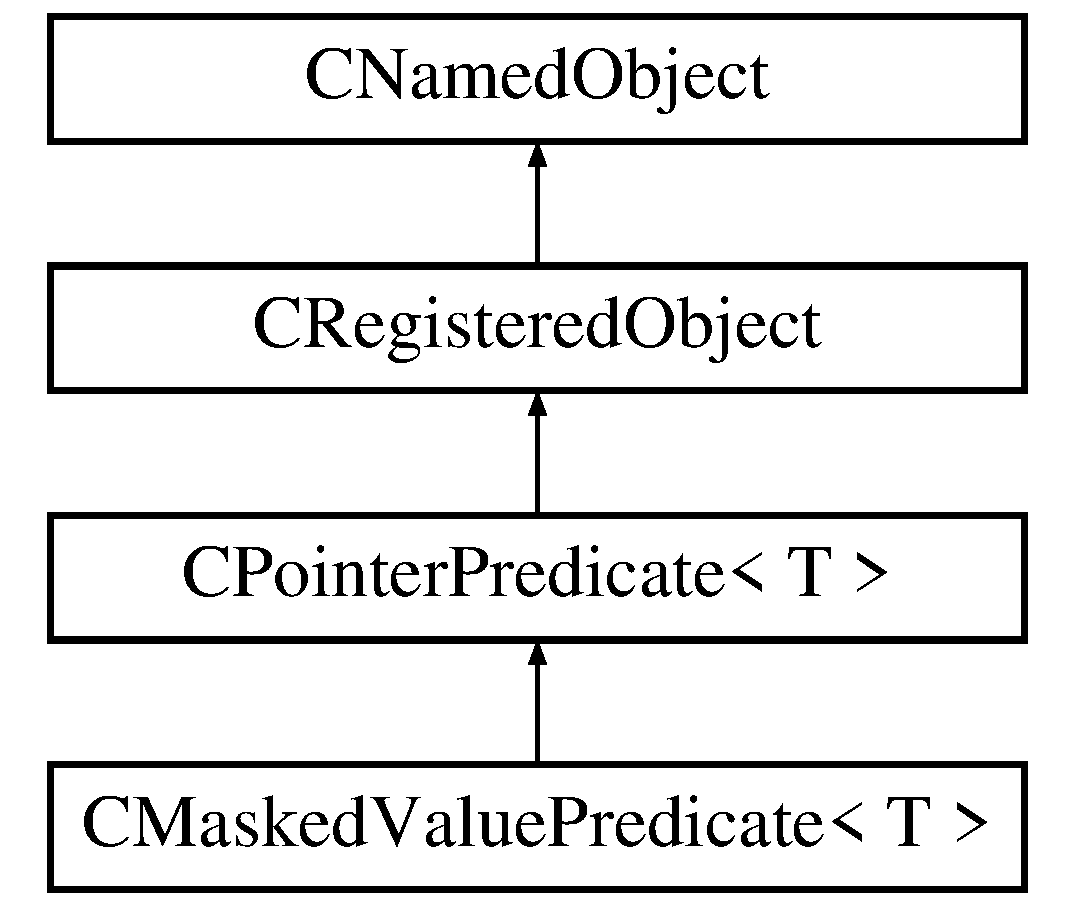
\includegraphics[height=4cm]{classCMaskedValuePredicate}
\end{center}
\end{figure}
\subsection*{Public Methods}
\begin{CompactItemize}
\item 
{\bf CMasked\-Value\-Predicate} (T am\_\-TValue, T am\_\-TMask={\bf COS\_\-ALLBITS})
\item 
{\bf CMasked\-Value\-Predicate} (const string \&r\-Name, T am\_\-TValue, T am\_\-TMask={\bf COS\_\-ALLBITS})
\item 
{\bf CMasked\-Value\-Predicate} (const char $\ast$p\-Name, T am\_\-TValue, T am\_\-TMask={\bf COS\_\-ALLBITS})
\item 
{\bf $\sim$CMasked\-Value\-Predicate} ()
\item 
int {\bf operator==} (const CMasked\-Value\-Predicate$<$ T $>$ \&a\-CMasked\-Value\-Predicate) const
\item 
T {\bf get\-Mask} () const
\item 
T {\bf get\-Value} () const
\item 
virtual bool {\bf operator()} (T n\-Value)
\item 
virtual string {\bf Describe\-Self} ()
\end{CompactItemize}
\subsection*{Protected Methods}
\begin{CompactItemize}
\item 
void {\bf set\-Mask} (const T am\_\-TMask)
\item 
void {\bf set\-Value} (const T am\_\-TValue)
\end{CompactItemize}
\subsection*{Private Methods}
\begin{CompactItemize}
\item 
{\bf CMasked\-Value\-Predicate} (const CMasked\-Value\-Predicate$<$ T $>$ \&a\-CMasked\-Value\-Predicate)
\item 
CMasked\-Value\-Predicate$<$ T $>$ {\bf operator=} (const CMasked\-Value\-Predicate$<$ T $>$ \&a\-CMasked\-Value\-Predicate)
\end{CompactItemize}
\subsection*{Private Attributes}
\begin{CompactItemize}
\item 
T {\bf m\_\-TValue}
\item 
T {\bf m\_\-TMask}
\end{CompactItemize}
\subsubsection*{template$<$typename T$>$ class CMasked\-Value\-Predicate$<$ T $>$}



\subsection{Constructor \& Destructor Documentation}
\index{CMaskedValuePredicate@{CMasked\-Value\-Predicate}!CMaskedValuePredicate@{CMaskedValuePredicate}}
\index{CMaskedValuePredicate@{CMaskedValuePredicate}!CMaskedValuePredicate@{CMasked\-Value\-Predicate}}
\subsubsection{\setlength{\rightskip}{0pt plus 5cm}template$<$typename T$>$ CMasked\-Value\-Predicate$<$ T $>$::CMasked\-Value\-Predicate (T {\em am\_\-TValue}, T {\em am\_\-TMask} = {\bf COS\_\-ALLBITS})\hspace{0.3cm}{\tt  [inline]}}\label{classCMaskedValuePredicate_a0}


The predicate mask \index{CMaskedValuePredicate@{CMasked\-Value\-Predicate}!CMaskedValuePredicate@{CMaskedValuePredicate}}
\index{CMaskedValuePredicate@{CMaskedValuePredicate}!CMaskedValuePredicate@{CMasked\-Value\-Predicate}}
\subsubsection{\setlength{\rightskip}{0pt plus 5cm}template$<$typename T$>$ CMasked\-Value\-Predicate$<$ T $>$::CMasked\-Value\-Predicate (const string \& {\em r\-Name}, T {\em am\_\-TValue}, T {\em am\_\-TMask} = {\bf COS\_\-ALLBITS})\hspace{0.3cm}{\tt  [inline]}}\label{classCMaskedValuePredicate_a1}


\index{CMaskedValuePredicate@{CMasked\-Value\-Predicate}!CMaskedValuePredicate@{CMaskedValuePredicate}}
\index{CMaskedValuePredicate@{CMaskedValuePredicate}!CMaskedValuePredicate@{CMasked\-Value\-Predicate}}
\subsubsection{\setlength{\rightskip}{0pt plus 5cm}template$<$typename T$>$ CMasked\-Value\-Predicate$<$ T $>$::CMasked\-Value\-Predicate (const char $\ast$ {\em p\-Name}, T {\em am\_\-TValue}, T {\em am\_\-TMask} = {\bf COS\_\-ALLBITS})\hspace{0.3cm}{\tt  [inline]}}\label{classCMaskedValuePredicate_a2}


\index{CMaskedValuePredicate@{CMasked\-Value\-Predicate}!~CMaskedValuePredicate@{$\sim$CMaskedValuePredicate}}
\index{~CMaskedValuePredicate@{$\sim$CMaskedValuePredicate}!CMaskedValuePredicate@{CMasked\-Value\-Predicate}}
\subsubsection{\setlength{\rightskip}{0pt plus 5cm}template$<$typename T$>$ CMasked\-Value\-Predicate$<$ T $>$::$\sim$CMasked\-Value\-Predicate ()\hspace{0.3cm}{\tt  [inline]}}\label{classCMaskedValuePredicate_a3}


\index{CMaskedValuePredicate@{CMasked\-Value\-Predicate}!CMaskedValuePredicate@{CMaskedValuePredicate}}
\index{CMaskedValuePredicate@{CMaskedValuePredicate}!CMaskedValuePredicate@{CMasked\-Value\-Predicate}}
\subsubsection{\setlength{\rightskip}{0pt plus 5cm}template$<$typename T$>$ CMasked\-Value\-Predicate$<$ T $>$::CMasked\-Value\-Predicate (const CMasked\-Value\-Predicate$<$ T $>$ \& {\em a\-CMasked\-Value\-Predicate})\hspace{0.3cm}{\tt  [private]}}\label{classCMaskedValuePredicate_c0}




\subsection{Member Function Documentation}
\index{CMaskedValuePredicate@{CMasked\-Value\-Predicate}!DescribeSelf@{DescribeSelf}}
\index{DescribeSelf@{DescribeSelf}!CMaskedValuePredicate@{CMasked\-Value\-Predicate}}
\subsubsection{\setlength{\rightskip}{0pt plus 5cm}template$<$typename T$>$ string CMasked\-Value\-Predicate$<$ T $>$::Describe\-Self ()\hspace{0.3cm}{\tt  [virtual]}}\label{classCMaskedValuePredicate_a8}


Operation Type: Selector

Purpose: Returns a string with the following information: 1 - m\_\-TMask 2 - m\_\-TValue 

Implements {\bf CPointer\-Predicate$<$ T $>$} {\rm (p.\,\pageref{classCPointerPredicate_a6})}.

Definition at line 315 of file CMasked\-Value\-Predicate.cpp.

References CMasked\-Value\-Predicate$<$ T $>$::m\_\-TMask, and CMasked\-Value\-Predicate$<$ T $>$::m\_\-TValue.\index{CMaskedValuePredicate@{CMasked\-Value\-Predicate}!getMask@{getMask}}
\index{getMask@{getMask}!CMaskedValuePredicate@{CMasked\-Value\-Predicate}}
\subsubsection{\setlength{\rightskip}{0pt plus 5cm}template$<$typename T$>$ T CMasked\-Value\-Predicate$<$ T $>$::get\-Mask () const\hspace{0.3cm}{\tt  [inline]}}\label{classCMaskedValuePredicate_a5}




Definition at line 352 of file CMasked\-Value\-Predicate.h.\index{CMaskedValuePredicate@{CMasked\-Value\-Predicate}!getValue@{getValue}}
\index{getValue@{getValue}!CMaskedValuePredicate@{CMasked\-Value\-Predicate}}
\subsubsection{\setlength{\rightskip}{0pt plus 5cm}template$<$typename T$>$ T CMasked\-Value\-Predicate$<$ T $>$::get\-Value () const\hspace{0.3cm}{\tt  [inline]}}\label{classCMaskedValuePredicate_a6}




Definition at line 357 of file CMasked\-Value\-Predicate.h.\index{CMaskedValuePredicate@{CMasked\-Value\-Predicate}!operator()@{operator()}}
\index{operator()@{operator()}!CMaskedValuePredicate@{CMasked\-Value\-Predicate}}
\subsubsection{\setlength{\rightskip}{0pt plus 5cm}template$<$typename T$>$ bool CMasked\-Value\-Predicate$<$ T $>$::operator() (T {\em n\-Value})\hspace{0.3cm}{\tt  [virtual]}}\label{classCMaskedValuePredicate_a7}


Operation Type: Override behavior

Purpose: Returns true if (n\-Value \& m\_\-TMask) == m\_\-TValue 

Implements {\bf CPointer\-Predicate$<$ T $>$} {\rm (p.\,\pageref{classCPointerPredicate_a5})}.

Definition at line 296 of file CMasked\-Value\-Predicate.cpp.

References CMasked\-Value\-Predicate$<$ T $>$::m\_\-TMask, and CMasked\-Value\-Predicate$<$ T $>$::m\_\-TValue.\index{CMaskedValuePredicate@{CMasked\-Value\-Predicate}!operator=@{operator=}}
\index{operator=@{operator=}!CMaskedValuePredicate@{CMasked\-Value\-Predicate}}
\subsubsection{\setlength{\rightskip}{0pt plus 5cm}template$<$typename T$>$ CMasked\-Value\-Predicate$<$T$>$ CMasked\-Value\-Predicate$<$ T $>$::operator= (const CMasked\-Value\-Predicate$<$ T $>$ \& {\em a\-CMasked\-Value\-Predicate})\hspace{0.3cm}{\tt  [private]}}\label{classCMaskedValuePredicate_c1}


\index{CMaskedValuePredicate@{CMasked\-Value\-Predicate}!operator==@{operator==}}
\index{operator==@{operator==}!CMaskedValuePredicate@{CMasked\-Value\-Predicate}}
\subsubsection{\setlength{\rightskip}{0pt plus 5cm}template$<$typename T$>$ int CMasked\-Value\-Predicate$<$ T $>$::operator== (const CMasked\-Value\-Predicate$<$ T $>$ \& {\em a\-CMasked\-Value\-Predicate}) const\hspace{0.3cm}{\tt  [inline]}}\label{classCMaskedValuePredicate_a4}




Definition at line 333 of file CMasked\-Value\-Predicate.h.

References CMasked\-Value\-Predicate$<$ T $>$::m\_\-TMask, CMasked\-Value\-Predicate$<$ T $>$::m\_\-TValue, and CPointer\-Predicate$<$ T $>$::operator==().\index{CMaskedValuePredicate@{CMasked\-Value\-Predicate}!setMask@{setMask}}
\index{setMask@{setMask}!CMaskedValuePredicate@{CMasked\-Value\-Predicate}}
\subsubsection{\setlength{\rightskip}{0pt plus 5cm}template$<$typename T$>$ void CMasked\-Value\-Predicate$<$ T $>$::set\-Mask (const T {\em am\_\-TMask})\hspace{0.3cm}{\tt  [inline, protected]}}\label{classCMaskedValuePredicate_b0}




Definition at line 365 of file CMasked\-Value\-Predicate.h.\index{CMaskedValuePredicate@{CMasked\-Value\-Predicate}!setValue@{setValue}}
\index{setValue@{setValue}!CMaskedValuePredicate@{CMasked\-Value\-Predicate}}
\subsubsection{\setlength{\rightskip}{0pt plus 5cm}template$<$typename T$>$ void CMasked\-Value\-Predicate$<$ T $>$::set\-Value (const T {\em am\_\-TValue})\hspace{0.3cm}{\tt  [inline, protected]}}\label{classCMaskedValuePredicate_b1}




Definition at line 370 of file CMasked\-Value\-Predicate.h.

\subsection{Member Data Documentation}
\index{CMaskedValuePredicate@{CMasked\-Value\-Predicate}!m_TMask@{m\_\-TMask}}
\index{m_TMask@{m\_\-TMask}!CMaskedValuePredicate@{CMasked\-Value\-Predicate}}
\subsubsection{\setlength{\rightskip}{0pt plus 5cm}template$<$typename T$>$ T CMasked\-Value\-Predicate$<$ T $>$::m\_\-TMask\hspace{0.3cm}{\tt  [private]}}\label{classCMaskedValuePredicate_o1}


The predicate value 

Definition at line 304 of file CMasked\-Value\-Predicate.h.

Referenced by CMasked\-Value\-Predicate$<$ T $>$::Describe\-Self(), CMasked\-Value\-Predicate$<$ T $>$::operator()(), and CMasked\-Value\-Predicate$<$ T $>$::operator==().\index{CMaskedValuePredicate@{CMasked\-Value\-Predicate}!m_TValue@{m\_\-TValue}}
\index{m_TValue@{m\_\-TValue}!CMaskedValuePredicate@{CMasked\-Value\-Predicate}}
\subsubsection{\setlength{\rightskip}{0pt plus 5cm}template$<$typename T$>$ T CMasked\-Value\-Predicate$<$ T $>$::m\_\-TValue\hspace{0.3cm}{\tt  [private]}}\label{classCMaskedValuePredicate_o0}




Definition at line 303 of file CMasked\-Value\-Predicate.h.

Referenced by CMasked\-Value\-Predicate$<$ T $>$::Describe\-Self(), CMasked\-Value\-Predicate$<$ T $>$::operator()(), and CMasked\-Value\-Predicate$<$ T $>$::operator==().

The documentation for this class was generated from the following files:\begin{CompactItemize}
\item 
{\bf CMasked\-Value\-Predicate.h}\item 
{\bf CMasked\-Value\-Predicate.cpp}\end{CompactItemize}
